\chapter{Computer music}

\section{Historical framework}\label{historical-framework}

First experiments in sound synthesis belong to the analogue era.

In the 1950s the study of the Cologne Radio (WDR) was in contrast to the GRM both in:

\begin{itemize}
\tightlist
\item terms of sound generation and manipulation techniques. 
\item terms of aesthetic positions.
\end{itemize}

The reference figure in this study was the composer Karheinz Stockhausen.

At that time his compositional ideas brought the strict rules of serialism into the generation of sound.

Every parameter of sound (pitch, spectrum, intensity, envelope, duration, etc.) was governed by rigid numerical rules.

The electroacoustic instruments available in the Cologne studio (oscillators, filters and ring modulators) and the possibility of recording the resulting sound on magnetic tape were the ideal tools for developing these ideas.

Karlheinz Stockhausen - Elektronische Studie II for tape (1954) - extract

Still in the electroacoustic field, a mix of the technical equipment of the two studios was found in the RAI Musical Phonology Studio in Milan where the composers of reference were Luciano Berio, Bruno Maderna and later Luigi Nono.

Their aesthetic positions were also less rigid than those of their French and German colleagues, mixing together different compositional techniques.

Bruno Maderna - Musica su due dimensioni for flute and tape (1958) - extract.

Computer music was born later for reasons obviously linked to the birth and development of digital technologies but it takes its cue from these (and other) electroacoustic experiences.

The first computer used for playing music was the CSIR Mk1 developed in Sydney in the late 1940s and presented at a public concert in 1951 where
it performed the piece \textit{Colonel Bogey March}.

Alan Turing was also working on primeval computer music in the summer of 1951 at the Computing Machine Laboratory in Manchester.

He and his collaborators produced three short melodic sequences played by the computer.

In the late 1950s Max Mathews was the most important computer scientist working at Bell Telephone Laboratories in New Jersey.

He worked primarily with mainframe computers made by IBM on several series of their MUSIC X program, a musical programming language that was upgraded over the next twenty years.

An early piece created in these studios was Beat Canon (1960) by J.R.Pierce (director of studio).

In 1963 the human voice was synthesized for the first time in these laboratories (speech synthesis).

Later musicians and engineers alike began to collaborate more on the making of music with computers creating more sophisticated work.

Aa example an exrept from `Lyric Variations' for Violin and Computer (1965-1968) by J.K.Randall.

In USA starting from the 60s artistic currents began to develop linked to the Studios and cultural environment where they arose.

\begin{itemize}
\item West coast \(\rightarrow\) \textit{Experimantal Music Studio MIT MEdia
  Laboratory} - Boston.

  Founded by Barry Vercoe in 1971, it develops software derived from the Music IV series on IBM 360 computers.

  In this studio Curtis Road created Computer Music Journal the world's leading computer music magazine.

  Composers such as James Dashow, Miller Puckette, Charles Dodge worked there, whose approach to composition was characterised by a strong structural rigor derived from the ideas developed by Stockhousen in Cologne.

  Three exemples:

  \begin{itemize}
  \item James Dashow - Conditional Assemblies for computer generated sounds (1980)
  \item Charles Dodge - The Waves for voice and electronics (1984)
  \item Curtis Road - `Granule' for computer generated sounds (1999)
  \end{itemize}
\item California two main poles:

  \begin{itemize}
  \tightlist
  \item Stanford University CCRMA (Karma) \(\rightarrow\) music production.
  \item San Diego University (CARU) and Lucas film studios \(\rightarrow\) software and hardware research.
  \end{itemize}

  The CCRMA was founded and directed by John Chowning, the inventor of FM synthesis and a leading figure in computer music.

  A figure of synthesis between technology and music, he addressed in each of his compositions a specific problem linked both to the synthesis of sound and to musical language.

  Through his work, which also took place in important European production centers such as IRCAM in Paris, he created a bridge between the two continents.

  An audio extracs from his work Turenas for computer generated sounds (1972) and a \href{img/turenas.pdf}{paper} about it.
\end{itemize}

\href{https://smcnetwork.org/centers.html}{Here} we can find a comprehensive list of computer music research and production centers.

\section{Randomness}\label{randomness}

Following or pursuing an random procedure means generating or transforming musical or acoustic material by integrating random choices into the decision-making process.

The concept of indeterminism affirms the denial of any determination of the will by external motives.

In our case a sequence of sonic events must be governed in whole or in part by chance or by a set of probabilities, regardless of the author's experience, taste, knowledge, and personality.

This makes it inevitable to rethink the composer's role in the creative act.

A reflection of this kind plays an important role in the poetics of American composer J. Cage who has often stated that his compositional principle is a departure from unity and a movement toward multiplicity:

\textit{ {[}\ldots{]} to abdicate one's subjectivity, to abandon one's own judgment to move toward the multiplicity that is life itself, of which man is but a small component, in the sea of constant variation
{[}\ldots{]}}

In Western musical tradition three different indeterministic procedures have been theorized and used.


\subsection{Chance }\label{chance}

The musical or sonic materials of the piece are:

\begin{itemize}
\item generated through random processes. 
\item fixed in symbolic form to allow a performance where the random elements fall within the limits of deterministic musical interpretation.
\end{itemize}

Two examples:

\begin{itemize}
\item The musical games in Europe between the second half of the 18th century and the beginning of the 19th century (C.Ph.E. Bach, F.J. Haydn, W.A. Mozart, etc.).

  \begin{itemize}
  \tightlist
  \item a set of musical bars that follow a harmonic scheme indexed and arranged by the composer in any order.
  \item use of a pair of dice to determine the order of performance (recomposition).
  \item the game allowed anyone even those with no musical knowledge to create harmonious and original pieces.
  \end{itemize}
  
  \begin{center}
  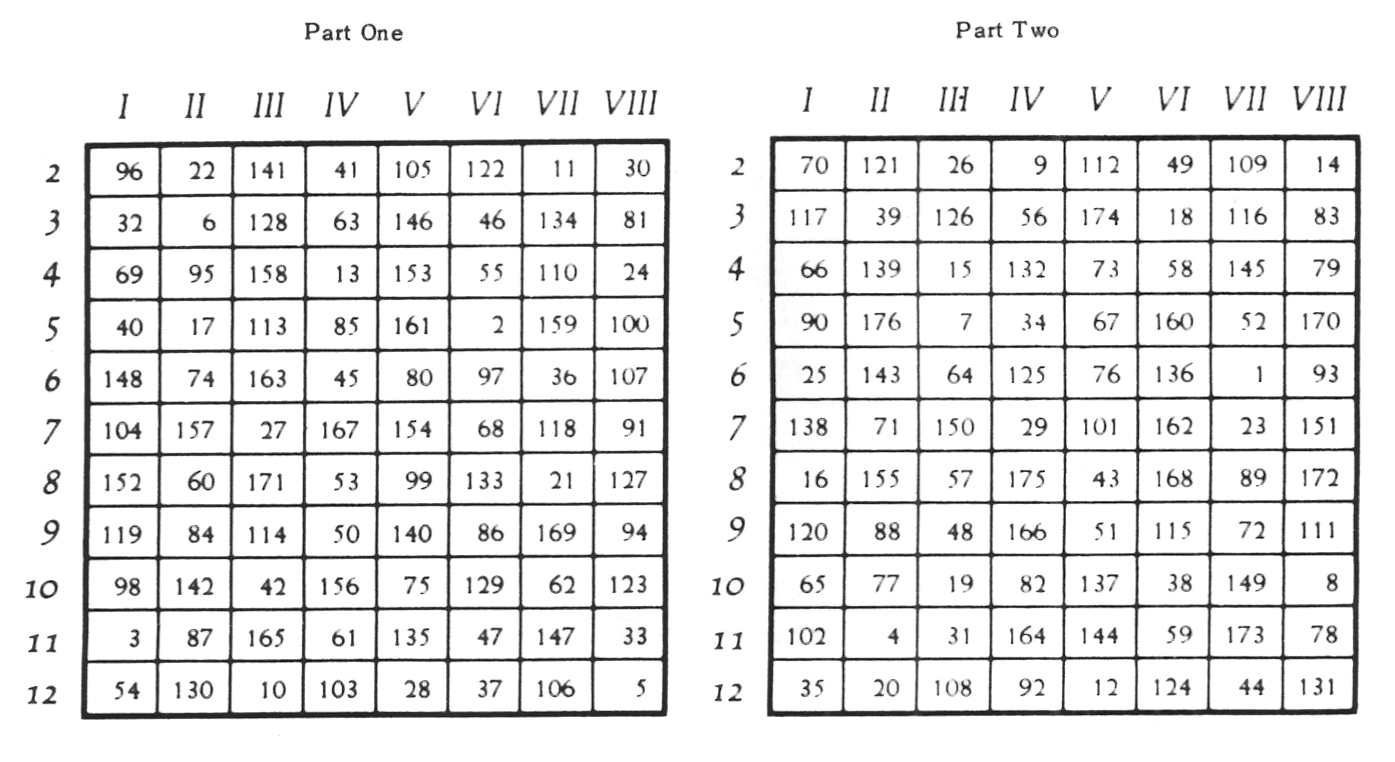
\includegraphics[scale=0.4]{../img/mozart_tables.png}
  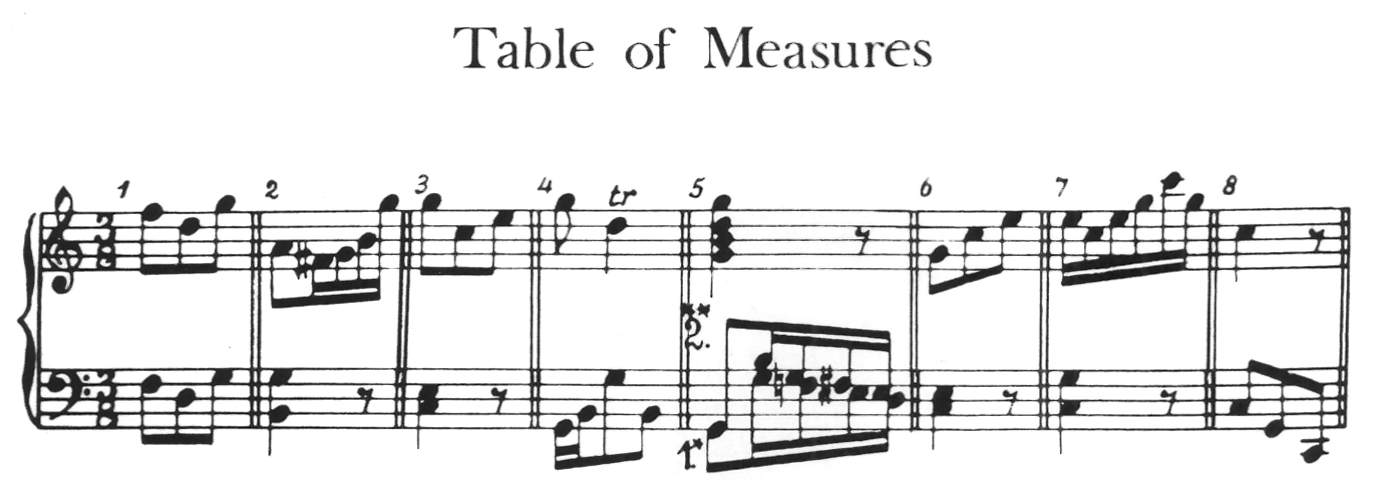
\includegraphics[scale=0.4]{../img/mozart_tables_1.png}
  \end{center}
  
\item Music of Changes by J.Cage for piano (1951) in which the formal structure, compositional method and choice of musical materials (pitches, dynamics and tempos) are determined by the roll of the dice of the I-Ching.

  \begin{itemize}
  \tightlist
  \item the collection consists of eight \textit{books} of music.
  \item to compile the score Cage used 8x8 grids (two-dimensional matrices) to facilitate correspondence with the 64 hexagrams of the I Ching.
  \item a first roll of the dice determines which sound event to write among those included in the sound grid, after which the next two rolls are dedicated to durations and dynamics.
  \end{itemize}
  
  \begin{center}
  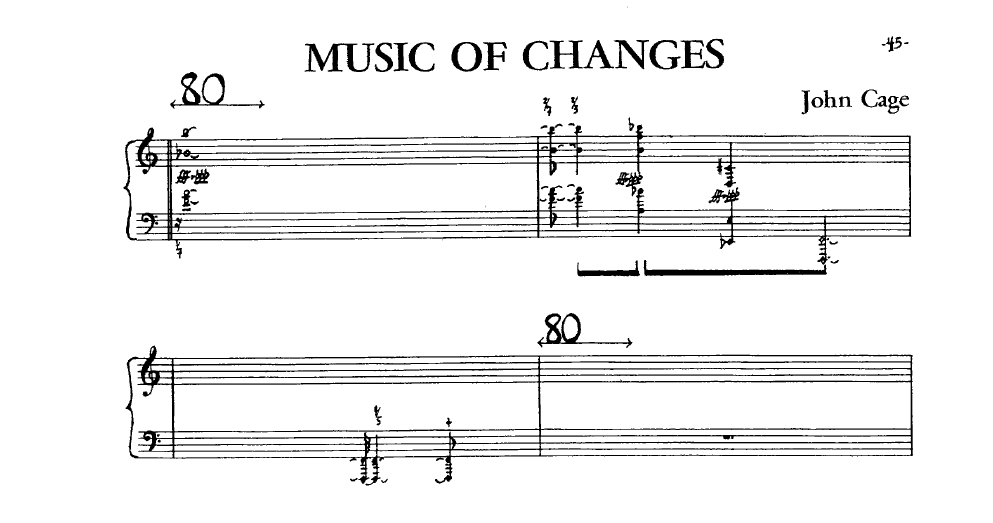
\includegraphics[scale=0.4]{../img/Music_O_C.png}
  \end{center}
\end{itemize}

\subsection{Indeterminacy}\label{indeterminacy}

It seeks the variable multiplicity of possible performances not chance.

Indeterminacy is the opposite of chance which adopts a method.

Chance relies on the logic of the method.

Indeterminacy relies on the performer's sensitivity.

It excludes the precise determination of certain parameters (pitch, duration, intensity, timbre) to give the performer a wide margin of freedom.

When taken to its extreme limits it ideally coincides with the opposite deterministic extreme: total improvisation or \textit{libero arbitrio}.

The concept of indeterminacy in music can be developed in two different ways:

\begin{enumerate}
\def\labelenumi{\arabic{enumi}.}
\tightlist
\item free choice of performance mode or form

  \begin{itemize}
  \tightlist
  \item Missa Cuiusvis Toni (1539) by Johannes Ockeghem.

    \begin{itemize}
    \tightlist
    \item the composer did not specify the clefs at the beginning of the staff.
    \item it can be performed in all four modes (Dorian, Phrygian, Lydian,  Mixolydian).
    \item the choice of which clef to use for reading (and therefore the mode) is left to the performers.
    \end{itemize}
    
    \begin{center}
    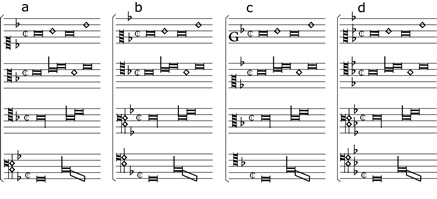
\includegraphics[scale=0.4]{../img/Cuiusvis_toni.png}
    \end{center}
  \item Serenata per un satellite (1969) by B. Maderna

    \begin{itemize}
    \tightlist
    \item It can be played by violin, flute (including piccolo), oboe (including oboe d'amore, even musette), clarinet (transposing the part, of course), marimba, harp, guitar, and mandolin (playing what they can), all together, individually, or in groups, improvising, in short, with the written notes.
    \item the whole piece should last between 4 and 12 minutes.
    \end{itemize}

    \begin{center}
    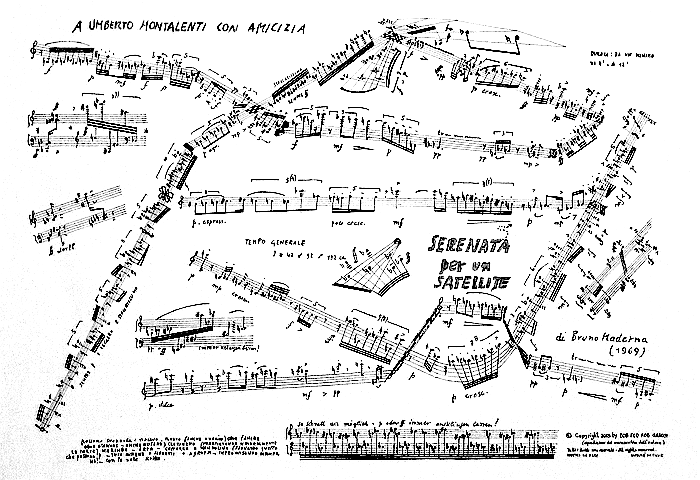
\includegraphics[scale=0.4]{../img/maderna_1.png}
    \end{center}
  \end{itemize}
\item graphic scores or verbal indications that suggest to the performer how the piece can be performed.

  \begin{itemize}
  \item December '52 by Earle Brown.
    \begin{center}
    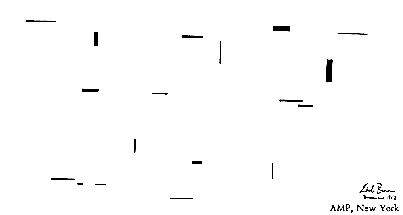
\includegraphics[scale=0.4]{../img/brown.png}
    \end{center}

  \item Intersection 3 by Morton Feldman (1964).
    \begin{center}
    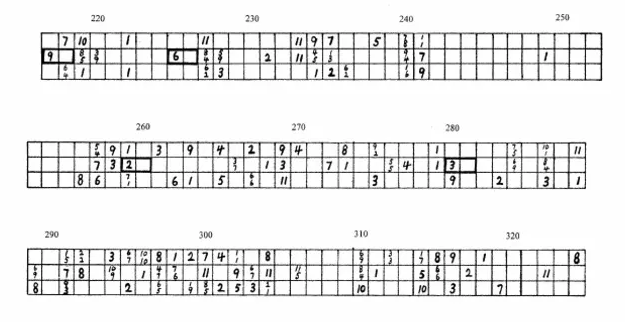
\includegraphics[scale=0.4]{../img/feld.png}
    \end{center}
    
  \item Intuitive Musik (1968) by K.Stockhausen
    \begin{center}
    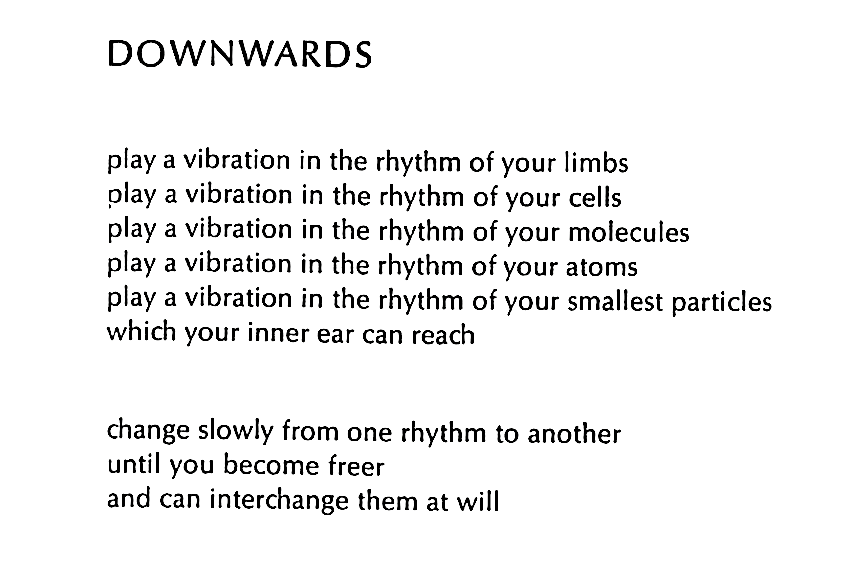
\includegraphics[scale=0.4]{../img/intu.png}
    \end{center}
  \item necessità espressive (Bruno Maderna)
  \end{itemize}
\end{enumerate}


\subsection{Alea}\label{alea}

These strategies became relatively common among composers of the European avant-garde after World War I.

Acousticist Werner Meyer-Eppler during the Darmstadt summer courses defined it this way:

\textit{A process can be defined as "aleatory" {[}\ldots{]} if its development
is established in general terms but depends on chance in the details}.

We explore the possible use of random procedures in SuperCollider using a SynthDef used in the previous chapter and then applying them to the sound synthesis techniques presented in this chapter and in the algorithmic composition procedures presented in the next chapter.

\begin{lstlisting}[frame=single] 
CICCIO
\end{lstlisting}

Let's define a Buffer and a SynthDef.

\begin{lstlisting}[frame=single] 
CICCIO
\end{lstlisting}

We can obtain random numbers in several ways, here the main objects.

\begin{itemize}
\tightlist
\item boolean \(\rightarrow\) 0.5.coin (0.0 = false, 1.0 = true, 0.x = probability). For example we can use it in a control structure to define the percentage of rests in a sequence.
\end{itemize}

\begin{lstlisting}[frame=single] 
CICCIO
\end{lstlisting}

\begin{itemize}
\tightlist
\item within a range (linear distribution) \(\rightarrow\) rrand(min, max). For example we can use it to define random positions in a Buffer.
\end{itemize}

\begin{lstlisting}[frame=single] 
CICCIO
\end{lstlisting}

\begin{itemize}
\tightlist
\item between 0 and max (linear distribution) \(\rightarrow\) rand(max). For example we can use it to define random amplitude.
\end{itemize}

\begin{lstlisting}[frame=single] 
CICCIO
\end{lstlisting}

\begin{itemize}
\tightlist
\item bipolar (linear distribution) \(\rightarrow\) rand2(+/- max)). For example we can use it to define random pan.
\end{itemize}

\begin{lstlisting}[frame=single] 
CICCIO
\end{lstlisting}

\begin{itemize}
\tightlist
\item choose in a finite set with a linear distribution \(\rightarrow\)
  {[}3,5,67,89{]}.choose. For example we can use it to define random
  choice among a set of durations.
\end{itemize}

\begin{lstlisting}[frame=single] 
CICCIO
\end{lstlisting}

There are other objects dedicated to nonlinear distributions but the principles on which they are based are the same as those just illustrated.

\section{Sound synthesis}\label{sound-synthesis}å

In this paragraph we will not delve into all the aspects of the individual synthesis techniques.

Only their main sonic and expressive possibilities related to composing music are focused.

Before starting let's define some utility:

\begin{itemize}
\tightlist
\item one SynthDef \(\rightarrow\) set of source signals. 
\item one SynthDef \(\rightarrow\) set of control signals (mouse, continuos). 
\item two audio bus to connect the source Synths with filters and FFT Synth. 
\item two control buses to control dynamically parameters (x, y and random signal values). 
\item one spectroscope.
\end{itemize}

\begin{lstlisting}[frame=single] 
CICCIO
\end{lstlisting}

\subsection{Additive}\label{additive}

With additive synthesis techniques we can realize: 

\begin{itemize}
\tightlist
\item harmonic spectra (pitched sounds). 
\item inharmonic spectra (non-pitched sounds).
\end{itemize}

Both categories can have:

\begin{itemize}
\tightlist
\item fixed spectrum.
\item variable spectrum.
\item spectral envelope.
\end{itemize}

There are different ways to do that.

\subsubsection{Wavetables}\label{wavetables}

Harmonic spectra or periodic noises.

Fixed spectrum.

\begin{enumerate}
\def\labelenumi{\arabic{enumi}.}
\item draw a single waveform period.
\item store it in a Buffer.
\item play it back at a defined frequency by an oscillator.
\end{enumerate}

The SynthDef.

\begin{lstlisting}[frame=single] 
CICCIO
\end{lstlisting}

We can paly it as in previous exemples.

\begin{itemize}
\tightlist
\item deterministic.
\end{itemize}

\begin{lstlisting}[frame=single] 
CICCIO
\end{lstlisting}

\begin{itemize}
\tightlist
\item random.
\end{itemize}

\begin{lstlisting}[frame=single] 
CICCIO
\end{lstlisting}

We can try to play them together.

Stop and kill.

\begin{lstlisting}[frame=single] 
CICCIO
\end{lstlisting}

\subsubsection{Vectorial}\label{vectorial}

This technique is a variant of wavetable lookup synthesis and allows the generation of variable spectra.

Harmonic spectra or periodic noises.

Variable spectrum.

\begin{enumerate}
\def\labelenumi{\arabic{enumi}.}
\tightlist
\item define an array of different waveforms.
\item during playback interpolate the reading dynamically with a control parameter.
\end{enumerate}

\begin{lstlisting}[frame=single] 
CICCIO
\end{lstlisting}

The SynthDef.

\begin{lstlisting}[frame=single] 
CICCIO
\end{lstlisting}

As usual we can change timbre parameter in four different ways.

\begin{enumerate}
\def\labelenumi{\arabic{enumi}.}
\tightlist
\item by sending single values (o to number of buses - 1).
\end{enumerate}

\begin{lstlisting}[frame=single] 
CICCIO
\end{lstlisting}

\begin{enumerate}
\def\labelenumi{\arabic{enumi}.}
\setcounter{enumi}{1}
\tightlist
\item by mapping a control signal on a control bus as argument.
\end{enumerate}

\begin{lstlisting}[frame=single] 
CICCIO
\end{lstlisting}

Change the control signal type and subaudio frequency.

\begin{lstlisting}[frame=single] 
CICCIO
\end{lstlisting}

Fade out and kill.

\begin{lstlisting}[frame=single] 
CICCIO
\end{lstlisting}

Another classic technique in digital synth design is to map the amplitude envelope with spectral modification.

A simulation of acoustic natural sounds.

\begin{lstlisting}[frame=single] 
CICCIO
\end{lstlisting}

\begin{lstlisting}[frame=single] 
CICCIO
\end{lstlisting}

Stop and kill.

\subsubsection{PWM}\label{pwm}

Pulse Width Modulation.

This technique is a variant of wavetable lookup synthesis and allows the generation of variable spectra.

Harmonic spectra.

Variable spectrum.

It is based on the concept of duty cycle.

\begin{center}
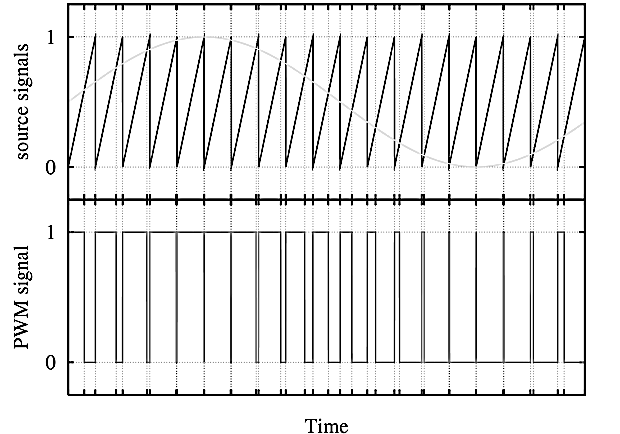
\includegraphics[scale=0.4]{../img/pwm.png}
\end{center}

By changing this parameter we modify the timbre.

The SynthDef.

\begin{lstlisting}[frame=single] 
CICCIO
\end{lstlisting}

The Synth.

\begin{lstlisting}[frame=single] 
CICCIO
\end{lstlisting}

We can change th duty cycle from 0.0 to 0.5.

Let's observe how the spectrum changes by set 1/3, 1/4, 1/5 etc.

\begin{lstlisting}[frame=single] 
CICCIO
\end{lstlisting}

The duty cycle and other parameter control methods are the same as those illustrated previously.

Stop and kill.

\begin{lstlisting}[frame=single] 
CICCIO
\end{lstlisting}

Some variations of this technique.

Blip \(\rightarrow\) classic pulse train derived from MusicN languages
(buzz) implemented in commercial synthesizers of the 90s.

We can define the number of harmonics as an argument.

The SynthDef.

\begin{lstlisting}[frame=single] 
CICCIO
\end{lstlisting}

The sequence.

\begin{lstlisting}[frame=single] 
CICCIO
\end{lstlisting}

Control signal.

\begin{lstlisting}[frame=single] 
CICCIO
\end{lstlisting}

Stop and kill:

\begin{lstlisting}[frame=single] 
CICCIO
\end{lstlisting}

We can also realize PWM with different waveforms stored in a Buffer (timbre stretching).

\begin{lstlisting}[frame=single] 
CICCIO
\end{lstlisting}

The Synths.

\begin{lstlisting}[frame=single] 
CICCIO
\end{lstlisting}

Fade out and kill.

\begin{lstlisting}[frame=single] 
CICCIO
\end{lstlisting}

\subsubsection{Classic}\label{classic}

Harmonic and inharmonic spectra.

Spectral envelope.

The techniques just described belong to the world of digital audio.

In the early electroacoustic music studios (Cologne and Milan), additive synthesis was achieved by recording each individual partial and then mixing it with the others.

Let's simulate this technique defining a SynthDef that play only one partial.

\begin{lstlisting}[frame=single] 
CICCIO
\end{lstlisting}

Then we can define spectra as Arrays and play it through a loop structure.

\begin{lstlisting}[frame=single] 
CICCIO
\end{lstlisting}

Deterministic sequence.

\begin{lstlisting}[frame=single] 
CICCIO
\end{lstlisting}

Random sequence - difference between chords and spectra.

\begin{lstlisting}[frame=single] 
CICCIO
\end{lstlisting}

Stop and kill.

\begin{lstlisting}[frame=single] 
CICCIO
\end{lstlisting}

\subsection{Subtractive}\label{subtractive}

Sound source ranging from white noise to rich spectra filtered by one or more filter(s).

The main types are:
\begin{enumerate}
\tightlist
\item Low Pass Filter (LPF) 
\item High Pass Filter (HPF) 
\item Band Pass Filter (BPF) 
\item Band Reject Filter (BRF) 
\item Resonant Filter (Resonz)
\end{enumerate}

In SuperCollider are all 2nd order Butterworth filters (-12 dB/oct).

We can control cut/central frequency (Hz).

In BPF, BRF and Resonz we can also control the bandwidth (reciprocal of Q).

\begin{enumerate}
\tightlist 
\item low values \(\rightarrow\) narrow band. 
\item high values \(\rightarrow\) wide band.
\end{enumerate}

Let's define:

\begin{enumerate}
\tightlist 
\item one SynthDef for signal source. 
    \begin{enumerate}
    \tightlist 
    \item we can switch among three types (0 = whitenoise, 1 = sawtoothwave, 2 = soundfile) 
    \item we can select the bus out.
    \end{enumerate} 
\item one SynthDef for each filter type.
    \begin{enumerate}
    \tightlist  
    \item we can select the bus in and the bus out.
    \end{enumerate}
\end{enumerate}

In SuperCollider there are many audio buses.

In a stereo system: 
\begin{enumerate}
\tightlist 
\item public buses \(\rightarrow\) 0 and 1 (L and R) 
\item private buses \(\rightarrow\) 2 and up.
\end{enumerate}

A simple signal flow.

\begin{center}
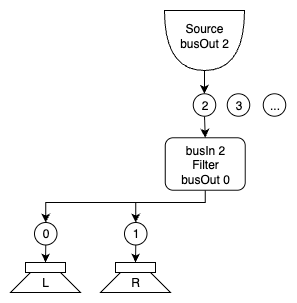
\includegraphics[scale=0.4]{../img/filt_1.png}
\end{center}

The SynthDefs.

\begin{lstlisting}[frame=single] 
CICCIO
\end{lstlisting}

Now we can test it.

The Synths (in right order).

\begin{lstlisting}[frame=single] 
CICCIO
\end{lstlisting}

Change the filter cutting frequency parameter in the usual ways.

\begin{lstlisting}[frame=single] 
CICCIO
\end{lstlisting}

Stop and kill.

\begin{lstlisting}[frame=single] 
CICCIO
\end{lstlisting}

We can sculpt the spectrum using filter banks in two combinations:

\begin{enumerate}
\def\labelenumi{\arabic{enumi}.}
\tightlist
\item series \(\rightarrow\) output of one filter is the input of the next until the public output.
\end{enumerate}

\begin{lstlisting}[frame=single] 
CICCIO
\end{lstlisting}

Stop it and kill.

\begin{lstlisting}[frame=single] 
CICCIO
\end{lstlisting}

\begin{enumerate}
\def\labelenumi{\arabic{enumi}.}
\setcounter{enumi}{1}
\tightlist
\item parallel \(\rightarrow\) output of source is the input of all filters, ouputs of filters mix together.
\end{enumerate}

\begin{lstlisting}[frame=single] 
CICCIO
\end{lstlisting}

\begin{lstlisting}[frame=single] 
CICCIO
\end{lstlisting}

In SuperCollider we have also pre builded filterbanks which can be used to simulate the resonant modes of an object.

The SynthDef.

\begin{lstlisting}[frame=single] 
CICCIO
\end{lstlisting}

The Synths.

\begin{lstlisting}[frame=single] 
CICCIO
\end{lstlisting}

Change resonator parameter.

\begin{lstlisting}[frame=single] 
CICCIO
\end{lstlisting}

Change source. 

\begin{enumerate}
\def\labelenumi{\arabic{enumi}.}
\setcounter{enumi}{1}
\tightlist
\item \(\rightarrow\) White Noise. 
\item \(\rightarrow\) Impulse
\item \(\rightarrow\) Dust.
\end{enumerate}

\begin{lstlisting}[frame=single] 
CICCIO
\end{lstlisting}

Fade out and kill.

\begin{lstlisting}[frame=single] 
CICCIO
\end{lstlisting}

\subsection{FM}\label{fm}

In additive synthesis and in some cases in subtractive synthesis the signals are added together to obtain complex spectra.

The computational cost is high since for each partial or filter we have to generate a UGen.

Through the different basic modulation techniques (RM, AM, FM and PM) we can obtain equally rich spectra with only two signals: 

\begin{enumerate}
\tightlist 
\item carrier 
\item modular
\end{enumerate}

In this paragraph we explore characteristics of frequency modulation (FM) which in its most basic form consists of using a rescaled sinusoidal control signal (modular) to dynamically vary the frequency of a sinusoid (carrier).

Three parameters:

\begin{enumerate}
\tightlist 
\item  carrier frequency (Hz). 
\item modular frequency \(\rightarrow\) MouseX from 2 to 500 Hz. 
\item deviation from carrier frequency (ampitude of modular signal) \(\rightarrow\) MouseY from 2 to 500 Hz.
\end{enumerate}

If the frequency of modular signal is sub audio and deviation is under \textasciitilde5 Hz \(\rightarrow\) \textit{vibrato effect}.

\begin{lstlisting}[frame=single] 
CICCIO
\end{lstlisting}

The Synth.

\begin{lstlisting}[frame=single] 
CICCIO
\end{lstlisting}

We can already recognize the characteristic sound of this technique.

Kill the Synth.

\begin{lstlisting}[frame=single] 
CICCIO
\end{lstlisting}

In classic FM algorithm we can control:

\begin{enumerate}
\tightlist 
\item modulation index \(\rightarrow\) quantity of modulation. 
\item harmonicity index \(\rightarrow\) quality of modulation.
\end{enumerate}

We can realize a lot of different sounds changing only these two parameters.

\begin{lstlisting}[frame=single] 
CICCIO
\end{lstlisting}

Let's explore it with mouse position.

\begin{lstlisting}[frame=single] 
CICCIO
\end{lstlisting}

Fade out and kill.

\begin{lstlisting}[frame=single] 
CICCIO
\end{lstlisting}

I suggest exploring the sonic potential of this technique empirically through mouse controls.

The x and y positions of the mouse could be dynamically reported in the Post window with \textit{.poll} method invoked on MouseX and MouseY UGens in \textit{ksig} SynthDef.

When we hear a sound that interests us we can write it down.

We can then recall them and eventually interpolate them with other sounds through envelopes or other.

One Example.

\begin{lstlisting}[frame=single] 
CICCIO
\end{lstlisting}

The Synths.

\begin{lstlisting}[frame=single] 
CICCIO
\end{lstlisting}

\subsection{FFT}\label{fft}

Some classical techniques related to the analysis and resynthesis of sound via the Fast Fourier Transform.

We analyze a signal by transforming it from time domain to frequency domain obtaining values of:

\begin{itemize}
\tightlist 
\item magnitude
\item phase
\end{itemize}

of a set of equidistant frequencies (bins) within the spectrum (think of them as the teeth of a comb).

We can manipulate these values in various ways and then bring them back into the time domain for playback.

There are two main procedures:

\begin{enumerate}
\tightlist 
\item analyze, process, and resynthesize a single signal. 
\item analyze two signals combine the data in various ways and resynthesize the result.
\end{enumerate}

In SuperCollider there ia a set of Classes dedicated to Phase Vocoder which is a historical FFT analysis and resynthesis technique.

To use classes in these examples download and install \href{https://supercollider.github.io/sc3-plugins/}{sc3-plugins}.

Be careful because FFT processes are CPU expensive.

\paragraph{Spectral Delay}\label{spectral-delay}

It differs from non-spectral delays in the fact that we can dynamically change delay time without pitch artefacts.

\begin{lstlisting}[frame=single] 
CICCIO
\end{lstlisting}

The Synths.

\begin{lstlisting}[frame=single] 
CICCIO
\end{lstlisting}

Fade out and kill.

\begin{lstlisting}[frame=single] 
CICCIO
\end{lstlisting}

\paragraph{BrickWall filter}\label{brickwall-filter}

Only bins above or below a threshold between +/-1 pass.

We can define ideal low and high pass filters.

\begin{lstlisting}[frame=single] 
CICCIO
\end{lstlisting}

The Synths.

\begin{lstlisting}[frame=single] 
CICCIO
\end{lstlisting}

Change filter freqs.

\begin{lstlisting}[frame=single] 
CICCIO
\end{lstlisting}

Dynamically (mouse x and y).

\begin{lstlisting}[frame=single] 
CICCIO
\end{lstlisting}

Fade out and kill.

\begin{lstlisting}[frame=single] 
CICCIO
\end{lstlisting}

\paragraph{Rect Comb filter}\label{rect-comb-filter}

Make gaps in spectrum.

\begin{enumerate}
\tightlist 
\item teeth \(\rightarrow\) number of teeth in the comb. 
\item fase \(\rightarrow\) starting phase of comb pulse. 
\item width \(\rightarrow\) pulse width of the comb.
\end{enumerate}

\begin{lstlisting}[frame=single] 
CICCIO
\end{lstlisting}

The Synths.

\begin{lstlisting}[frame=single] 
CICCIO
\end{lstlisting}

Change phases.

\begin{lstlisting}[frame=single] 
CICCIO
\end{lstlisting}

Change width and teeth dynamically.

\begin{lstlisting}[frame=single] 
CICCIO
\end{lstlisting}

Fade out and kill.

\begin{lstlisting}[frame=single] 
CICCIO
\end{lstlisting}

\paragraph{Mag Smear}\label{mag-smear}

Average magnitudes across bins.

We can set the number of bins to average on each side of bin.

\begin{lstlisting}[frame=single] 
CICCIO
\end{lstlisting}

The Synths.

\begin{lstlisting}[frame=single] 
CICCIO
\end{lstlisting}

Fade out and kill.

\begin{lstlisting}[frame=single] 
CICCIO
\end{lstlisting}

\paragraph{Freeze}\label{freeze}

Freeze magnitudes when freeze argument \textgreater{} 0.

\begin{lstlisting}[frame=single] 
CICCIO
\end{lstlisting}

The Synths and the sequence.

\begin{lstlisting}[frame=single] 
CICCIO
\end{lstlisting}

\paragraph{Cross synthesys.}\label{cross-synthesys.}

There are several cross-synthesis techniques.

In this example, the bins of signal A are replaced by those of signal B.

\begin{lstlisting}[frame=single] 
CICCIO
\end{lstlisting}

The Synths (two different sources).

\begin{lstlisting}[frame=single] 
CICCIO
\end{lstlisting}

\begin{lstlisting}[frame=single] 
CICCIO
\end{lstlisting}

\section{Algorithmic structures}\label{algorithmic-structures}

In this chapter we expanded our sonic vocabulary.

We can now design formal structures by adopting the same strategies illustrated in the previous chapter or through non-deterministic algorithms.

Let's give an example of this second case.

Let's suppose we want to create a piece with dreamlike feeling based on three musical objects:

\begin{enumerate}
\def\labelenumi{\arabic{enumi}.}
\setcounter{enumi}{1}
\tightlist
\item a continuos changing crystal sound (filter bank). 
\item a percussive brilliant sound (vector synth). 
\item a strange piano (FFT filter).
\end{enumerate}

Let's design the first.

Define one SynthDef and a function that design the musical object.
\begin{enumerate}
\tightlist
\item random spectra.
\item random duration.
\item random release.
\end{enumerate}

\begin{lstlisting}[frame=single] 
CICCIO
\end{lstlisting}

Turns the musical object on and off randomly.

Test it.

\begin{lstlisting}[frame=single] 
CICCIO
\end{lstlisting}

Kill it.

\begin{lstlisting}[frame=single] 
CICCIO
\end{lstlisting}

Let's design the second in the same manner.

\begin{itemize}
\tightlist
\item random pitch from a set.
\item random rythm.
\item random amplitudes.
\item random sequence activation.
\item random pan.
\end{itemize}

\begin{lstlisting}[frame=single] 
CICCIO
\end{lstlisting}

Turns the musical object on and off randomly.

\begin{lstlisting}[frame=single] 
CICCIO
\end{lstlisting}

Kill it.

\begin{lstlisting}[frame=single] 
CICCIO
\end{lstlisting}

Let's design the third musical object.

\begin{lstlisting}[frame=single] 
CICCIO
\end{lstlisting}

Test it.

\begin{lstlisting}[frame=single] 
CICCIO
\end{lstlisting}

Kill it.

\begin{lstlisting}[frame=single] 
CICCIO
\end{lstlisting}

We can now put it all together in a score that turns different combinations on and off randomly.

\begin{lstlisting}[frame=single] 
CICCIO
\end{lstlisting}

At each performance the piece will be a little different in its form but will always maintain the characteristics that we had set ourselves.

This is a simple example for explanatory reasons but it is clear how through this process we can arrive at designing extremely complex structures and forms.

\section{Composition sketches proposal}\label{composition-sketches-proposal}

Create a musical work using the instruments and the procedure just described.

Suggestions: 

\begin{itemize}
\tightlist
\item research other synthesis techniques or delve deeper into some of them. 
\item modify the contents of the proposed SynthDefs based on your musical parameter control needs. 
\item explore algorithms that dynamically modify the form through random control structures such as if, case, and switch (search for help files). 
\item verify how and how much random parameters can influence the realization of the initial musical idea.
\end{itemize}